\documentclass[tikz]{standalone}
\begin{document}
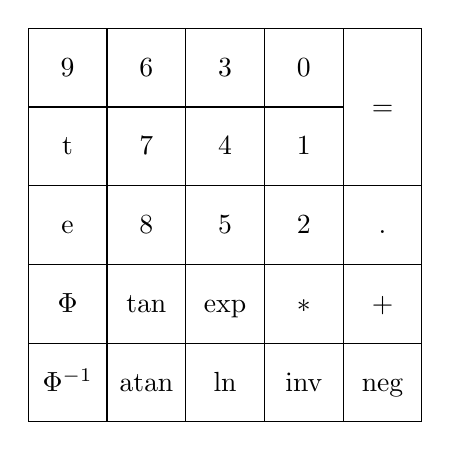
\begin{tikzpicture}
\draw (0,0) rectangle (5,5);
\draw (0,0) grid (4,5);
\draw (0,0) grid (5,3);
\foreach \x/\y/\n in {
  0/0/$\Phi^{-1}$,
  1/0/atan,
  2/0/ln,
  3/0/inv,
  4/0/neg,
  0/1/$\Phi$,
  1/1/tan,
  2/1/exp,
  3/1/$*$,
  4/1/$+$,
  0/2/e,
  1/2/8,
  2/2/5,
  3/2/2,
  4/2/.,
  0/3/t,
  1/3/7,
  2/3/4,
  3/3/1,
  0/4/9,
  1/4/6,
  2/4/3,
  3/4/0,
  4/3.5/=%
}
\draw (\x+0.5,\y+0.5) node {\smash{\n}\vphantom{t}};
\end{tikzpicture}
\end{document}

Note that angles start at "downward" and go clockwise (like the sun).
Note that `tan` takes as input tau-angles, where 0 = 0deg and 1 = 360deg